%ankicard
%ankitags mathematics algebra precalculus
\subsection{Distance of two points on the Real Line}
%ankifront
\begin{small}
    \begin{tabularx}{1\textwidth}{
            p{\dimexpr1\textwidth\relax}
        }
        \toprule
        \textbf{Distance of two points on the Real Line} \\
        \bottomrule
    \end{tabularx}
\end{small}
%ankifront end

%ankiback

% \begin{small}
\begin{tabularx}{1\textwidth}{
        p{\dimexpr0.5\textwidth\relax}
        p{\dimexpr0.5\textwidth\relax}
    }
\toprule
\multicolumn{2}{c}{\textbf{Distance between two points}} \\
\midrule

$ d(a, b) = \left| b - a \right| $ &
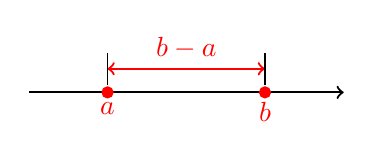
\begin{tikzpicture}
    % Draw the line
    \draw[thick, ->] (0,0) -- (4,0);
    
    % Draw points
    \filldraw[red] (1,0) circle (2pt) node[below] {$a$};
    \filldraw[red] (3,0) circle (2pt) node[below] {$b$};
    
    % Draw the vector
    \draw[red, thick, <->] (1,0.3) -- (3,0.3) node[midway, above] {$ \lvert b - a \rvert $};
    \draw[black] (1,0.1) -- ++(0,0.4);
    \draw[black] (3,0.1) -- ++(0,0.4);
    % \draw[red, thick, <-] (0,-0.2) -- (4,-0.2);
\end{tikzpicture}
\\
\bottomrule


\end{tabularx}
% \end{small}
%ankiback end
